\documentclass{beamer}
\usetheme{metropolis}
\usepackage{listings}
\usepackage{amsfonts}
\usepackage{dsfont}
\usepackage{amsmath}
\usepackage{bbm}
\usepackage{verbatim}
%\usepackage{tipa}
\usepackage{tikz}
\usetikzlibrary{fit}
\usepackage{color}
\usepackage{booktabs}
\usepackage{tipa}
\usepackage{amssymb}
\usepackage{verbatim}
\usepackage[absolute,overlay]{textpos}
\usepackage{pifont}% http://ctan.org/pkg/pifont
\newcommand{\cmark}{\ding{51}}%
\newcommand{\xmark}{\ding{55}}%
\usetikzlibrary{bayesnet}
\usetikzlibrary{decorations.markings}
\usetikzlibrary{decorations.pathmorphing}
\tikzset{squiggle/.style={decorate, decoration={snake,amplitude=.4mm}}}
\usepackage{xcolor}
\definecolor{pop1}{HTML}{1F78b4}
\definecolor{pop2}{HTML}{164C13}
\definecolor{pop3}{HTML}{d95F02}
\definecolor{orange}{HTML}{d95F02}
\definecolor{teal}{HTML}{1b9e77}
\newcommand{\pop}[1]{\textcolor{pop1}{#1}}
\newcommand{\popp}[1]{\textcolor{pop2}{#1}}
\newcommand{\tree}[1]{\textcolor{pop3}{#1}}
\newcommand{\orange}[1]{\textcolor{orange}{#1}}
\newcommand{\teal}[1]{\textcolor{teal}{#1}}


\newcommand{\nextForm}[1]{\rotatebox[origin=c]{270}{$_{\curvearrowright}$}$_{#1}$}
 
\usepackage{amsfonts}
\usepackage{tabularx}
%\usepackage{color}
\usepackage{graphicx}
\usepackage{booktabs}
\usepackage{xcolor}
\usepackage{tikz}
\usetikzlibrary{trees}
\usetikzlibrary{fit}
\usetikzlibrary{calc}
\usetikzlibrary{bayesnet}
\usepackage[absolute,overlay]{textpos}
\usepackage{stmaryrd}
\newcommand{\sem}[1]{\llbracket #1\rrbracket}
\newcommand{\tuple}[1]{\ensuremath{\left \langle #1\right \rangle}}
\usepackage{booktabs}
\usepackage{tipa}
\usepackage{amssymb}
\usepackage{verbatim}
\usepackage[absolute,overlay]{textpos}
\usepackage{pifont}% http://ctan.org/pkg/pifont
\newcommand{\cmark}{\ding{51}}%
\newcommand{\xmark}{\ding{55}}%
\usetikzlibrary{bayesnet}
\usetikzlibrary{decorations.markings}

\newcommand\Wider[2][3em]{%
\makebox[\linewidth][c]{%
  \begin{minipage}{\dimexpr\textwidth+#1\relax}
  \raggedright#2
  \end{minipage}%
  }%
}


\usepackage[utf8]{inputenc}

\usepackage{amssymb}% http://ctan.org/pkg/amssymb
\usepackage{pifont}% http://ctan.org/pkg/pifont

\usepackage{fancyvrb}

\usepackage[most]{tcolorbox}
\definecolor{block-gray}{gray}{0.10}
\newtcolorbox{mycode}{colback=block-gray,grow to right by=0mm,grow to left
by=0mm, boxrule=0pt,boxsep=0pt,breakable,fontupper=\color{white}}

%% Program ::=
%%   (if Bool List
%%     (append RecursiveList
%%             RecursiveList
%%             RecursiveList))
%% RecursiveList ::= List
%%          | (recurse List)

            
\begin{SaveVerbatim}[]{ListSketch}
Bool ::= (<= Int) | (>= Int)
       | (= Int)
Int  ::= 0
       | (+1 Int) | (-1 Int)
       | (length List)
       | (head List)
List ::= nil | X
       | (filter Bool List)
       | (tail List)
       | (list Int)
\end{SaveVerbatim}

\begin{SaveVerbatim}[]{ListSketchFull}
Program ::= (if (Bool Int)
                List
                (append RecursiveList
                        RecursiveList
                        RecursiveList))
RecursiveList ::= List
                | (recurse List)
Bool ::= (<= Int) | (>= Int)
       | (= Int)
Int  ::= 0
       | (+1 Int) | (-1 Int)
       | (length List)
       | (head List)
List ::= nil | X
       | (filter Bool List)
       | (tail List)
       | (list Int)
\end{SaveVerbatim}

\begin{SaveVerbatim}[]{Reverse}
(if (<= (+1 0) (length X))
    X
    (append (recurse (tail X))
            (list (head X))))
\end{SaveVerbatim}
\begin{SaveVerbatim}[]{Reversep}
(if (= (+1 0) (length X))
    X
    (append (recurse (filter (<= (+1 0)) (tail X)))
            (list (head X))))
\end{SaveVerbatim}

\begin{SaveVerbatim}[]{Count}
(length (filter (= (head X)) (tail X)))
\end{SaveVerbatim}

\begin{SaveVerbatim}[]{Countp}
(-1 (length (filter (= (head X)) X)))
\end{SaveVerbatim}

\begin{SaveVerbatim}[]{Sort}
(if (<= (+1 0) (length X))
    X
    (append (recurse (filter (<= (head X)) (tail X)))
            (list (head X))
            (recurse (filter (>= (head X)) (tail X)))))
\end{SaveVerbatim}

\begin{SaveVerbatim}[]{Sortp}
(if (= (+1 0) (length X))
    X
    (append (recurse (tail X))
            (list (length X))))
\end{SaveVerbatim}

\begin{SaveVerbatim}[]{TextSketch}
Program ::= Term
          | Program + Term
Term    ::= String
          | substr(Pos,Pos)
Pos     ::= Number
          | pos(Str,Str,Num)
Num     ::= 0 | 1 | 2 | ... 
          | -1 | -2 | ...
Str     ::= Character 
          | Character + String
Character ::= a | b | c | ...
\end{SaveVerbatim}

\newcommand{\theSystem}{\textsc{ProgramSample}}
\usepackage{arydshln}

\newcommand{\Expect}{\mathds{E}} %{{\rm I\kern-.3em E}}
\newcommand{\Probability}{\mathds{P}} %{{\rm I\kern-.3em P}}

\DeclareMathOperator*{\argmax}{arg\,max}
%Information to be included in the title page:
\title{Growing libraries of concepts with wake-sleep program induction}
\author{Kevin Ellis \& Mathias Sabl\'e Meyer\\Joint with: Lucas Morales, Armando Solar-Lezama, Joshua B. Tenenbaum\\Heavy inspiration from: Eyal Dechter}
\institute{MIT} 
%\date{November 2017}
  
 
\begin{document}
 
\frame{\titlepage}

\begin{frame}{The Language of Thought}
\begin{tikzpicture}
    \node at (-3,1) {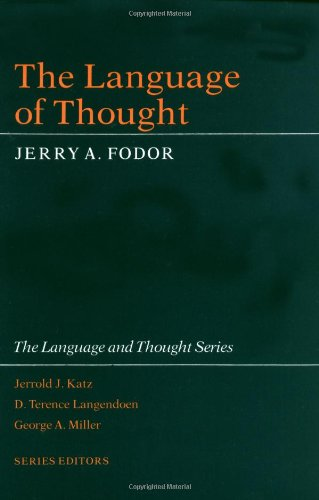
\includegraphics[width = 6cm]{Fodor.jpg}};
  \node at (2,2) {
\includegraphics[width = 8cm]{Solomon.png}};
%
    \end{tikzpicture}
\end{frame}

\begin{frame}{Engineering the language of thought}
 \begin{tikzpicture}
    \node () {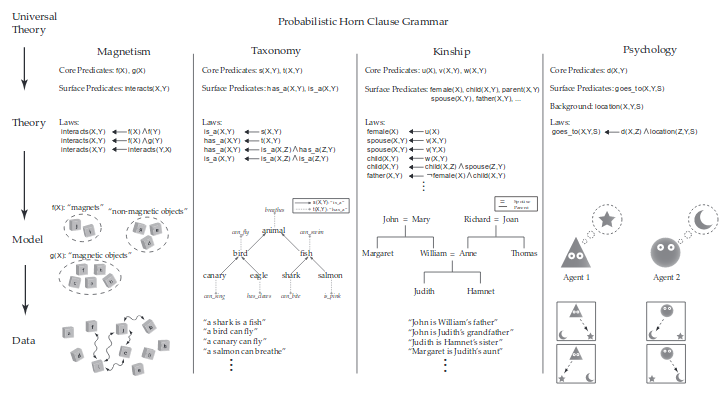
\includegraphics[width = 15.6cm]{theory.png}};
    \node at (-5,-4) {  Ullman et al 2012};
    \end{tikzpicture}
\end{frame}

\begin{frame}{Engineering the language of thought}
  \begin{tikzpicture}
    \node at(0,0) {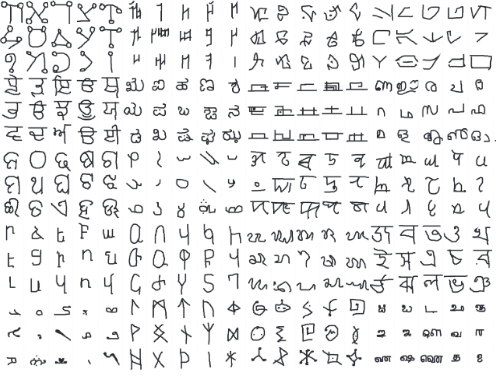
\includegraphics[width = 8cm]{characters.png}};
    \node at(-3,2) {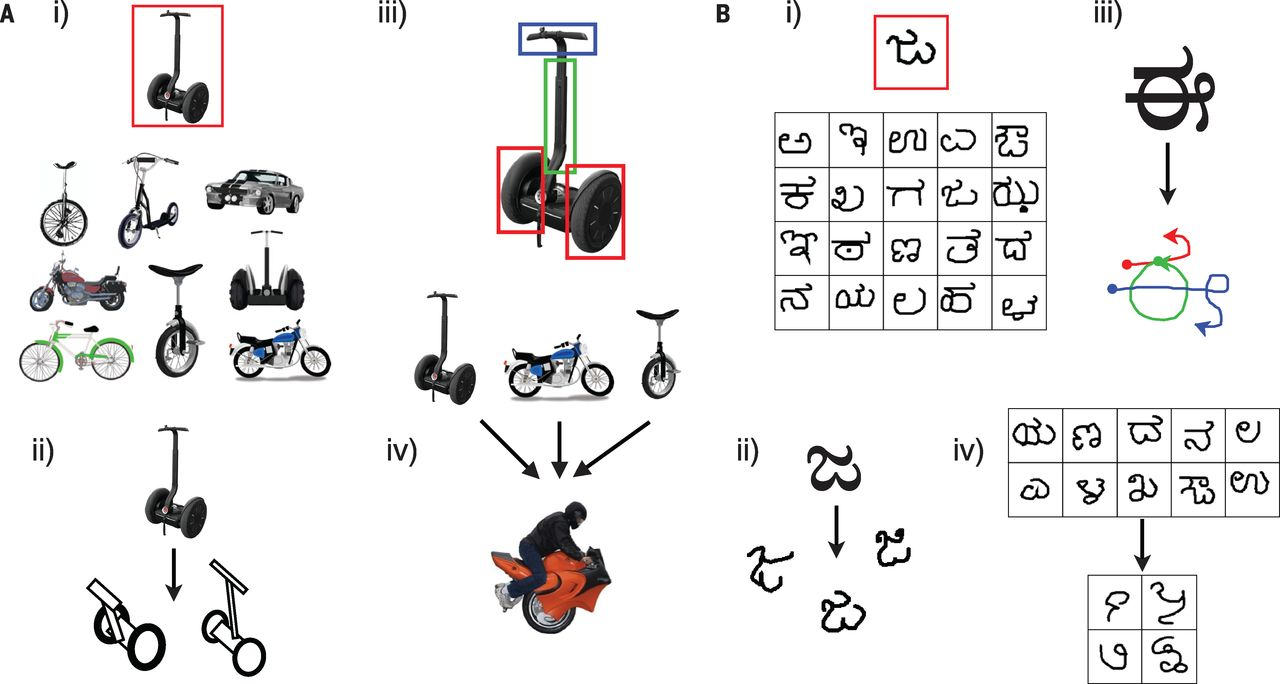
\includegraphics[width = 8cm]{Brendan.jpg}};

    \node at (-5,-4) {  Lake et al 2015};
    \end{tikzpicture}
\end{frame}





\begin{frame}{Growing a domain-specific language of thought}
  
  %  \Large
  Goal: acquire domain-specific knowledge needed to induce a class of programs


  
  \pause
  \vspace{1cm}

  \begin{itemize}
  \item Library of concepts (declarative knowledge)
    \item Search strategy (procedural knowledge)
    \end{itemize}
\end{frame}

\begin{frame}{DSL: Library of concepts}
\Wider[5.4em]{
  \renewcommand\code\texttt
  \renewcommand\codechar[1]{\texttt{"#1"}}
  \newcommand{\helpSize}{0.25cm}
  \footnotesize\begin{tabular}{cc}
    \toprule
Tasks and     \pop{Programs} & DSL\\
    \midrule
      \begin{tabular}{cc}
        \begin{tabular}{c}
          \code{[7\, 2\, 3]}$\to$\code{[7\, 3]}         \\
          \code{[1\, 2\, 3\, 4]}$\to$\code{[3\, 4]} \\
          \code{[4\, 3\, 2\, 1]}$\to$\code{[4\, 3]} \\
          \pop{\code{$f(\ell) = $}\code{($f_1$ $\ell$ ($\lambda$ (x)}}\\
          \hspace{1.15cm}\pop{\code{(> x 2)))}}       \\
          \\
          \\
          \code{[2\, 7\, 8\, 1]}$\to $\code{8}               \\
          \hspace{0.15cm}\code{[3\, 19\, 14]}$\to $\code{19}                \\
          \pop{\code{$f(\ell) = $}\code{($f_2$ $\ell$)}}
        \end{tabular}
        &
        \hspace{-0.3cm}\begin{tabular}{c}
          \code{[7\, 3]}$\to $\code{False}                              \\
          \hspace{0.3cm}\code{[3]}$\to $\code{False}                    \\
          \hspace{-0.3cm}\code{[9\, 0\, 0]}$\to $\code{True\phantom{e}} \\
          \hspace{0.3cm}\code{[0]}$\to $\code{True\phantom{e}}                        \\
          \hspace{-0.3cm}\code{[0\, 7\, 3]}$\to $\code{True\phantom{e}}                \\
          \pop{\code{$f(\ell) = $}\code{($f_3$ $\ell$ 0)}}
        \end{tabular}
      \end{tabular}
    &
    \begin{tabular}{l}
      \popp{$f_0(\ell,$\code{r}$) \,=\, $\code{(foldr r $\ell$ cons)}}\\
      \hspace{\helpSize}($f_0$: \emph{Append lists }\code{r}\emph{ and  $\ell$})\\
      \popp{$f_1(\ell,$\code{p}$) \,=\, $\code{(foldr $\ell$ nil ($\lambda$ (x a)}}\\
      \hspace{0.5cm}\popp{\code{(if (p x) (cons x a) a)))}}\\
      \hspace{\helpSize}($f_1$: \emph{Higher-order filter function})\\
      %(lambda (fold $0 0 (lambda (lambda (if (gt? $0 $1) $0 $1)))))
      \popp{$f_2(\ell) \,=\, $\code{(foldr $\ell$ 0 ($\lambda$ (x a)}}\\
      \popp{\phantom{$f_2(\ell) \,=\, $}\code{(if (> a x) a x)))}}\\
      \hspace{\helpSize}($f_2$: \emph{Maximum element in list $\ell$})\\
      \popp{$f_3(\ell,$\code{k}$) \,=\, $\code{(foldr $\ell$ (is-nil $\ell$)}}\\
      \phantom{$f_1(\ell,$}
      \popp{\code{($\lambda$ (x a) (if a a (= k x))))}}\\
      \hspace{\helpSize}($f_2$: \emph{Whether $\ell$ contains }\code{k})\\
    \end{tabular}
  \\\bottomrule
  \end{tabular}
}
\end{frame}

\begin{frame}{DreamCoder}
  \begin{itemize}
  \item   \textbf{Wake:} Solve problems by writing programs
  \item \textbf{Sleep:} Improve DSL and neural recognition model:
    \begin{itemize}
    \item \textbf{Sleep-G:} Improve DSL (\textbf{G}enerative model)
      \item \textbf{Sleep-R:} Improve \textbf{R}ecognition model
      \end{itemize}
  \end{itemize}
  Combines ideas from Wake-Sleep \& Exploration-Compression algorithm by Eyal Dechter


\end{frame} 

\begin{frame}[t]{DSL learning as Bayesian inference}
  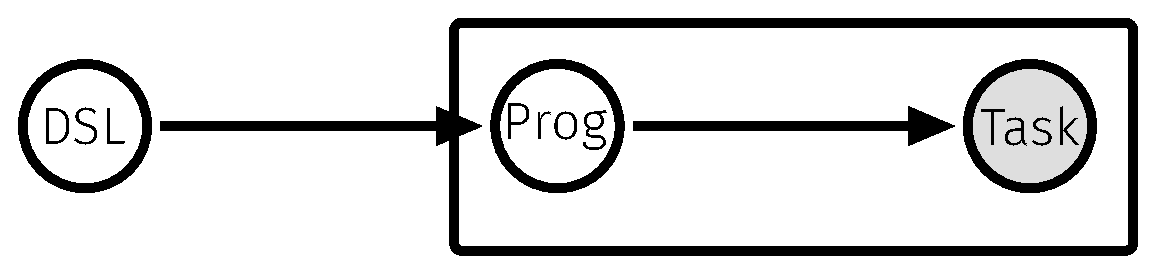
\includegraphics[width = 11cm]{figures/animation/EC.eps}

\vspace{1cm}
  
  \textbf{[Dechter et al., 2013]}  [Liang et al, 2010]; [Lake et al, 2015]

  \vfill
  Gray: Observed.\\
  White: Latent.\\
  Boxed (plate): Repeated.\\
  
\end{frame}
\begin{frame}[t]{DSL learning as \alert{amortized} Bayesian inference}
  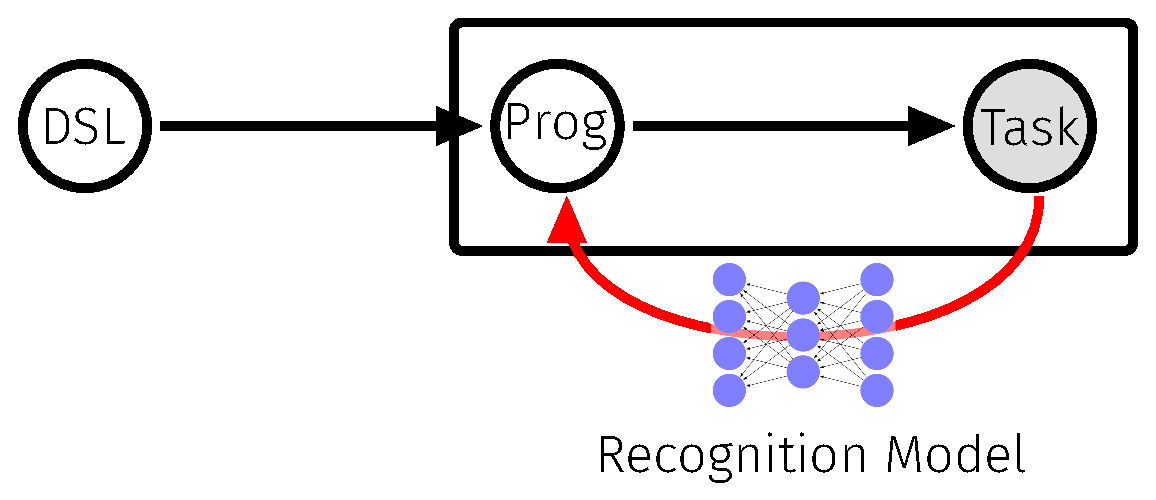
\includegraphics[width = 11cm]{figures/animation/DC.eps}

  \vfill
  Recognition model: Neural net.\\
  Red: Bottom-up inference.\\
  Gray: Observed.\\
  White: Latent.\\
  Boxed (plate): Repeated.\\

\end{frame}
\begin{frame}[t]{Wake: Problem solving}
  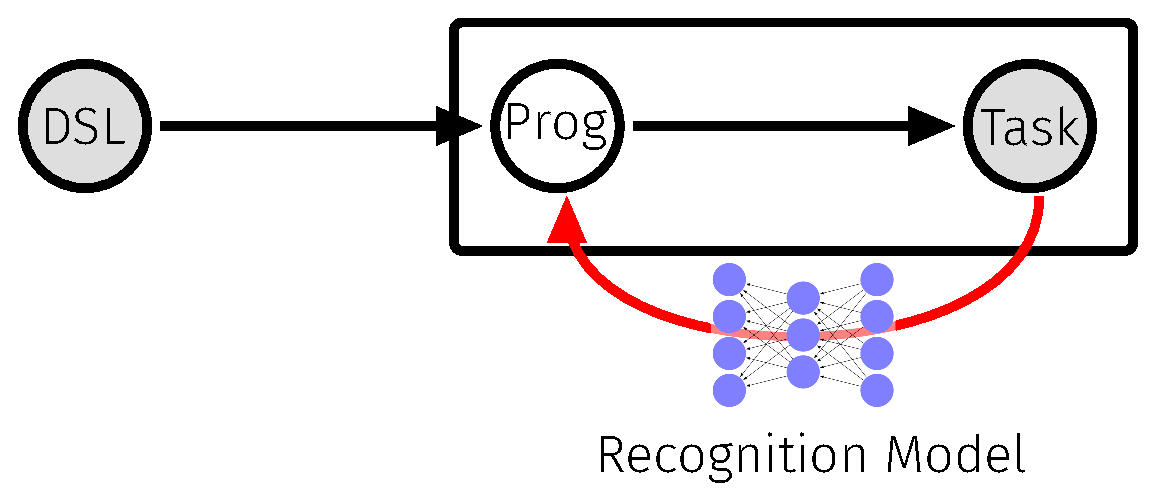
\includegraphics[width = 11cm]{figures/animation/Wake.eps}

    \vfill
  Recognition model: Neural net.\\
  Red: Bottom-up inference.\\
  Gray: Observed.\\
  White: Latent.\\
  Boxed (plate): Repeated.\\

\end{frame}
\begin{frame}[t]{Sleep-G: Memory consolidation}
  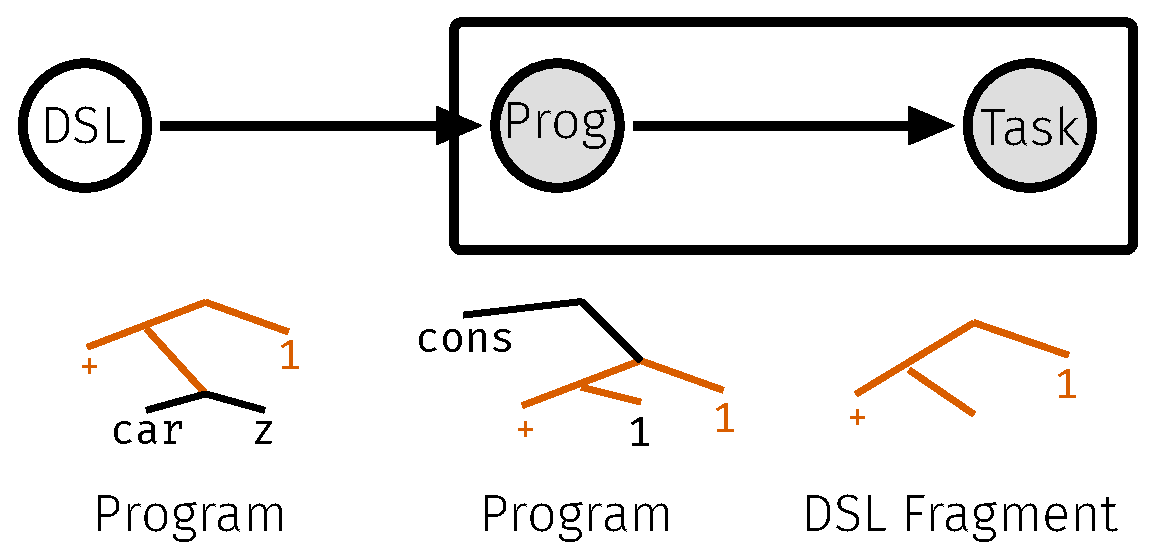
\includegraphics[width = 11cm]{figures/animation/Sleep-G.eps}
  \vfill
  \textbf{Fragment Grammars: O'Donnell 2015.}\\
  Orange: Code fragments.\\
  %% Gray: Observed.\\
  %% White: Latent.\\
  %% Boxed (plate): Repeated.\\

  
\end{frame}
\begin{frame}[t]{Sleep-R: Experience replay}
  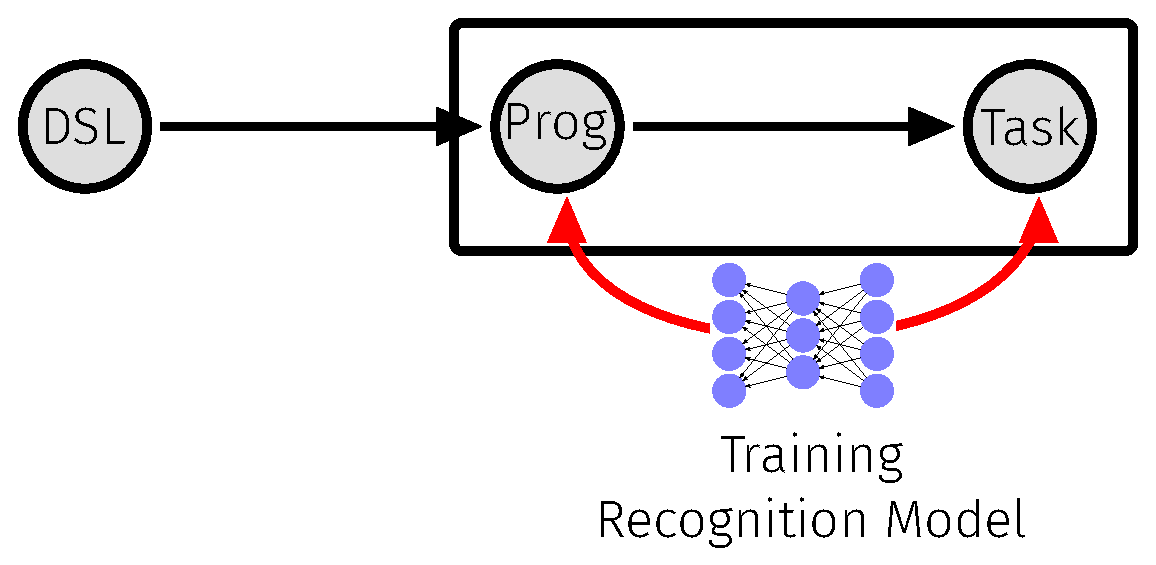
\includegraphics[width = 11cm]{figures/animation/Sleep-R-1.eps}
\end{frame}
\begin{frame}[t]{Sleep-R: Dreaming}
  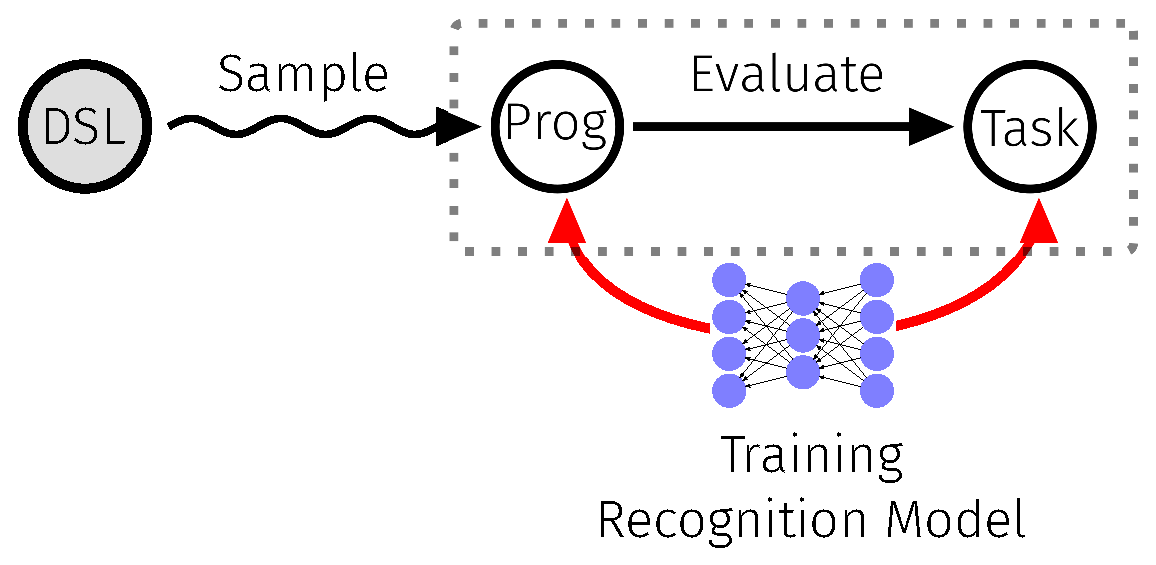
\includegraphics[width = 11cm]{figures/animation/Sleep-R-2.eps}

\end{frame}




\begin{frame}{List functions --- \small{Created \& investigated by Lucas
  Morales}}


  \vspace{1cm}
  
  \begin{figure}[b]\centering
\vspace{-0.5cm}  \begin{tabular}{lll}
    \toprule
    Name & Input & Output \\\midrule
    repeat-3 & [7\, 0] & [7\, 0\, 7\, 0\, 7\, 0] \\
    drop-3 & [0\, 3\, 8\, 6\, 4] & [6\, 4] \\
    rotate-2 & [8\, 14\, 1\, 9] & [1\, 9\, 8\, 14] \\
    count-head-in-tail & [1\, 2\, 1\, 1\, 3] & 2 \\
    keep-div-5 & [5\, 9\, 14\, 6\, 3\, 0] & [5\, 0] \\
    product & [7\, 1\, 6\, 2] & 84 \\
    \bottomrule
  \end{tabular}
  %\captionof{table}{Some tasks in our list function domain.}\label{listExamples}\vspace{-0.5cm}
\end{figure}

  Discovers 38 concepts, including `filter'
\end{frame}

\begin{frame}{List functions: Learning curves on hold out tasks}

  \begin{center}
      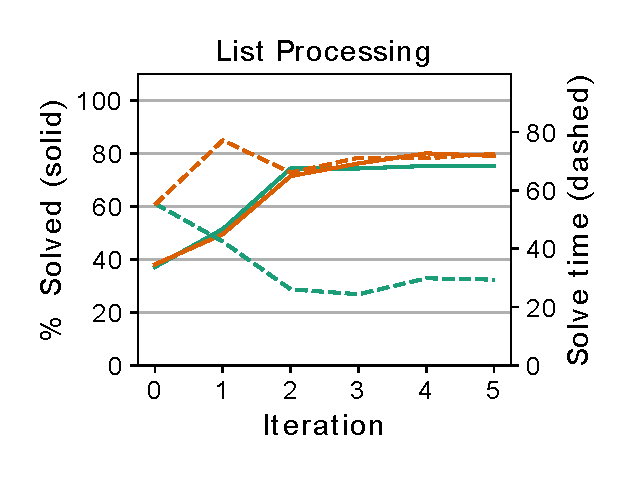
\includegraphics[width = 6.5cm]{figures/listLearningCurve.eps} 
    \end{center}

Learning curves for DreamCoder both with (\orange{in orange}) and without
    (\teal{in teal}) the recognition model. Solid lines: \% holdout testing tasks solved w/ 10m timeout. Dashed lines: Average solve time, averaged only over tasks that are solved.


  \end{frame}

%% \begin{frame}{Text editing}
%%   In the style of FlashFill (Gulwani 2012)

%%   \centering  \includegraphics[width = 5cm]{textColumn.png}

%%   SyGuS problems: solves 3\% before learning, vs 74\% after learning. Best prior work: 80\%

  

%%   \end{frame}

%% \begin{frame}{Symbolic regression from visual input}
%% \centering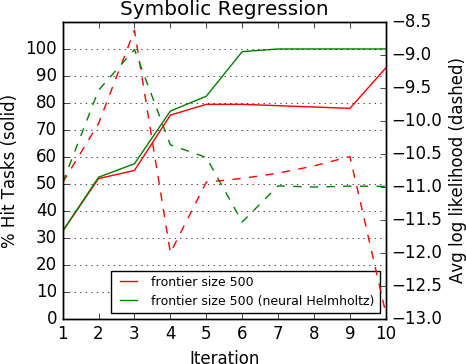
\includegraphics[width = 5cm]{symbolicRegression.png}
%% \end{frame}

\begin{frame}{Turtle graphics --- \small{Created \& investigated by Mathias
  Sablé--Meyer}}

  \begin{block}{DSL}
    \texttt{OP ::= FW x | RT x | UP | DOWN | SET state}
  \end{block}

  \begin{block}{Tasks}
    \texttt{task : unit -> image}
  \end{block}

  \vspace{0.2cm}

  \only<1>{
    \begin{columns}[T]
      \column{0.5 \textwidth}
        \begin{mycode}
          \texttt{FW 1}\\
          \vspace*{5\baselineskip}
        \end{mycode}
      \column{0.5 \textwidth}
        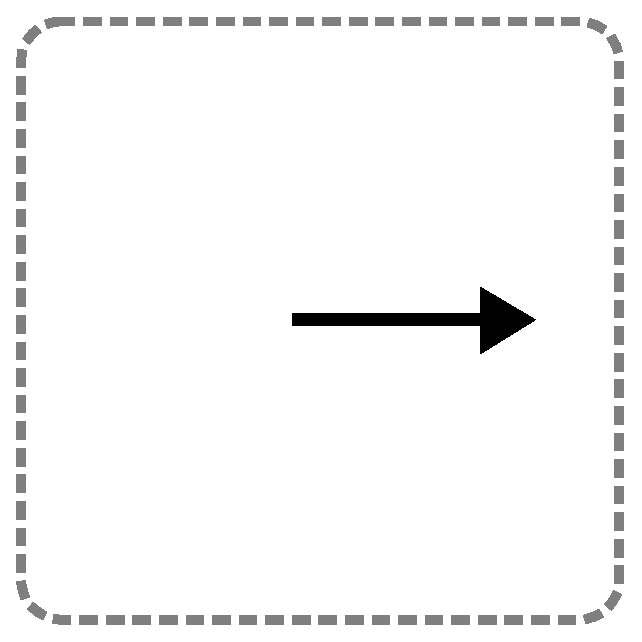
\includegraphics[width = 4cm]{figures/teachLogo/line.eps}
    \end{columns}
  }
  \only<2>{
    \begin{columns}[T]
      \column{0.5 \textwidth}
        \begin{mycode}
          \texttt{FW 1}\\
          \texttt{RT} $\frac\pi2$\\
          \texttt{FW 1}\\
          \vspace*{3\baselineskip}
        \end{mycode}
      \column{0.5 \textwidth}
        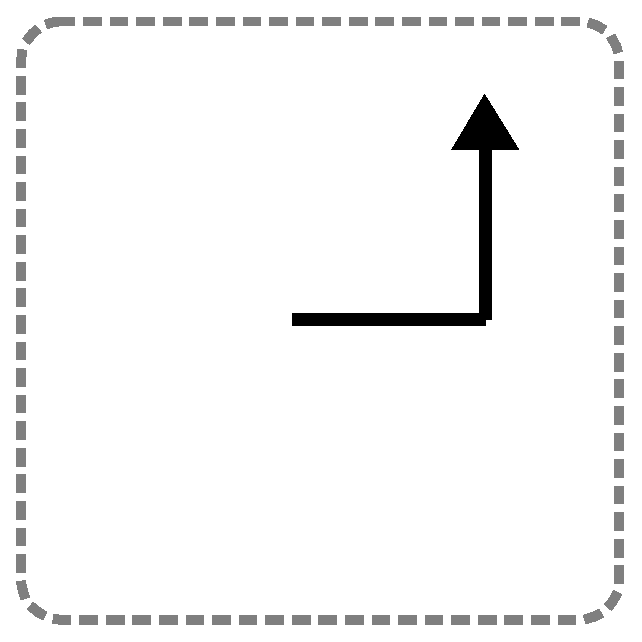
\includegraphics[width = 4cm]{figures/teachLogo/angle.eps}
    \end{columns}
  }
  \only<3>{
    \begin{columns}[T]
      \column{0.5 \textwidth}
        \begin{mycode}
          \texttt{FW 1}\\
          \texttt{RT} $\frac\pi2$\\
          \texttt{FW 1}\\
          \texttt{RT} $\frac\pi2$\\
          \texttt{FW 1}\\
          \vspace*{1\baselineskip}
        \end{mycode}
      \column{0.5 \textwidth}
        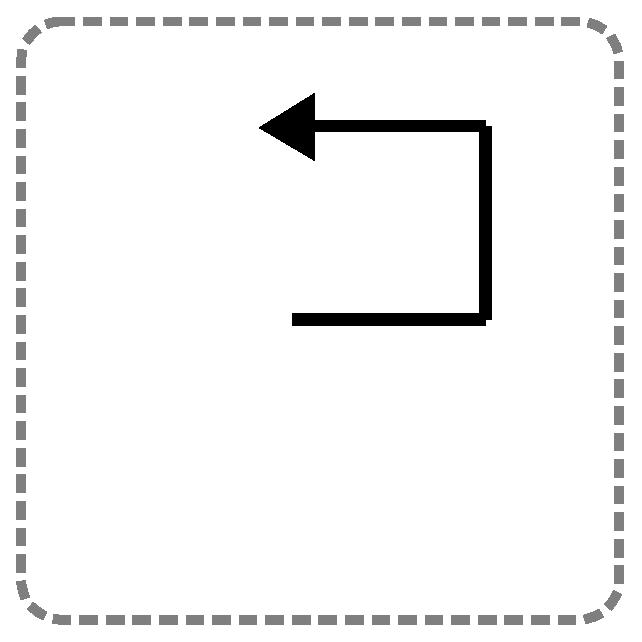
\includegraphics[width = 4cm]{figures/teachLogo/angle2.eps}
    \end{columns}
  }
  \only<4>{
    \begin{columns}[T]
      \column{0.5 \textwidth}
        \begin{mycode}
          \texttt{for i in range(4)}\\
          \texttt{> FW 1}\\
          \texttt{> RT} $\frac\pi2$\\
          \vspace*{3\baselineskip}
        \end{mycode}
      \column{0.5 \textwidth}
        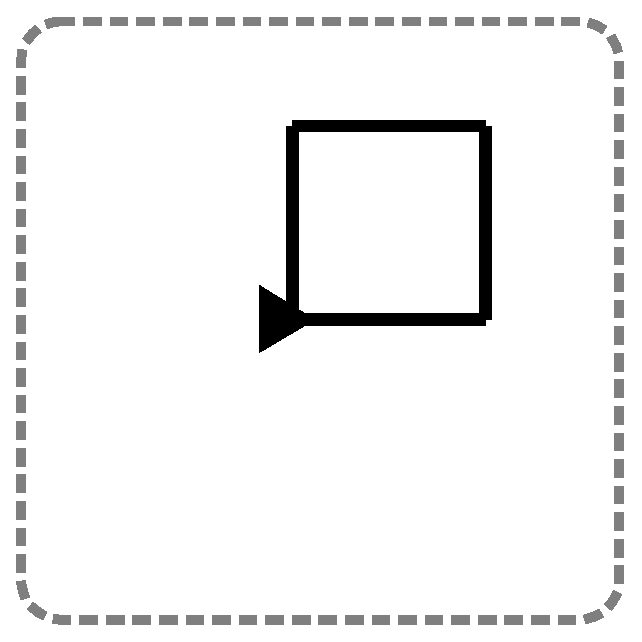
\includegraphics[width = 4cm]{figures/teachLogo/square.eps}
    \end{columns}
  }
  \only<5>{
    \begin{columns}[T]
      \column{0.5 \textwidth}
        \begin{mycode}
          \texttt{for i in range(8)}\\
          \texttt{> FW 1} \\
          \texttt{> SET origin} \\
          \texttt{> RT} $\frac{2\pi}{8}$\\
          \vspace*{2\baselineskip}
        \end{mycode}
      \column{0.5 \textwidth}
        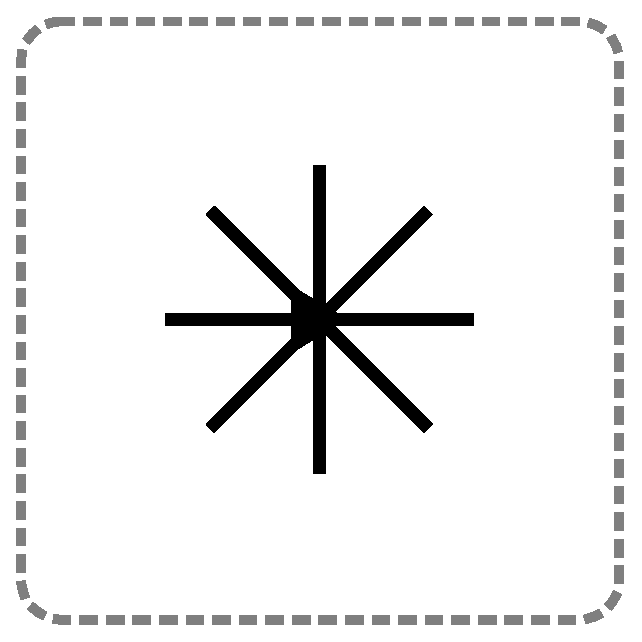
\includegraphics[width = 4cm]{figures/teachLogo/star.eps}
    \end{columns}
  }
  \only<6>{
    \begin{columns}[T]
      \column{0.5 \textwidth}
        \begin{mycode}
          \texttt{for i in range(8)}\\
          \texttt{> PU} \\
          \texttt{> FW} $\frac{\text{\texttt{i}}}{2}$\\
          \texttt{> PD} \\
          \texttt{> FW} $\frac{\text{\texttt{i}}}{2}$\\
          \texttt{> RT} $\frac\pi2$\\
          \vspace*{0\baselineskip}
        \end{mycode}
      \column{0.5 \textwidth}
        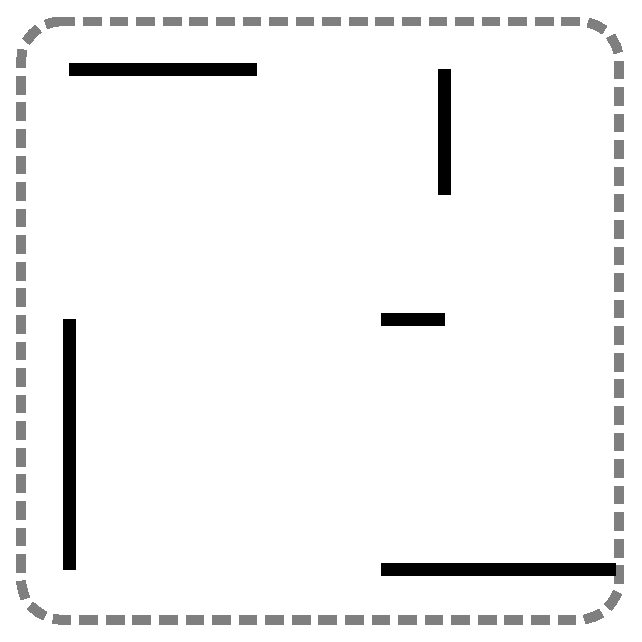
\includegraphics[width = 4cm]{figures/teachLogo/spiral.eps}
    \end{columns}
  }
  \only<7>{
    \begin{columns}[T]
      \column{0.5 \textwidth}
        \begin{mycode}
          \texttt{for i in range($\infty$)}\\
          \texttt{> FW $\varepsilon$}\\
          \texttt{> RT} $\varepsilon$\\
          \vspace*{3\baselineskip}
        \end{mycode}
      \column{0.5 \textwidth}
        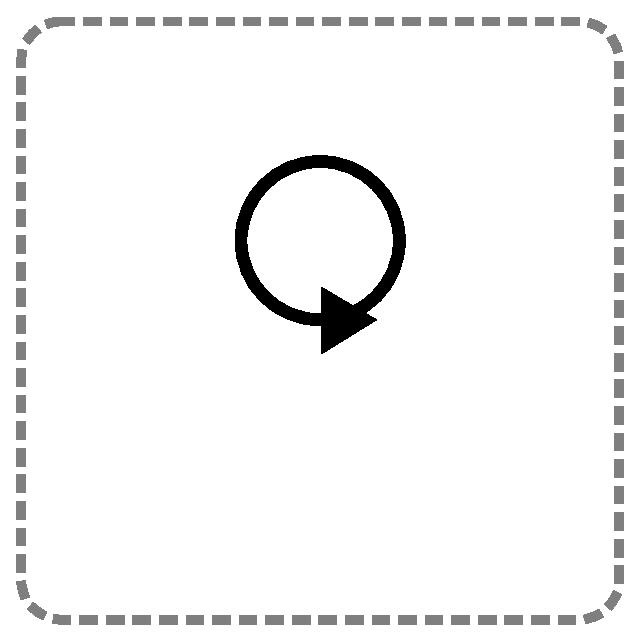
\includegraphics[width = 4cm]{figures/teachLogo/circle.eps}
    \end{columns}
  }
  \only<8-9>{
    \begin{columns}[T]
      \column{0.5 \textwidth}
        \begin{mycode}
          \texttt{for i in range($5\times\infty$)}\\
          \texttt{> FW $\text{\texttt{i}}\times\varepsilon$}\\
          \texttt{> RT} $\varepsilon$\\
          \vspace*{3\baselineskip}
        \end{mycode}
      \column{0.5 \textwidth}
        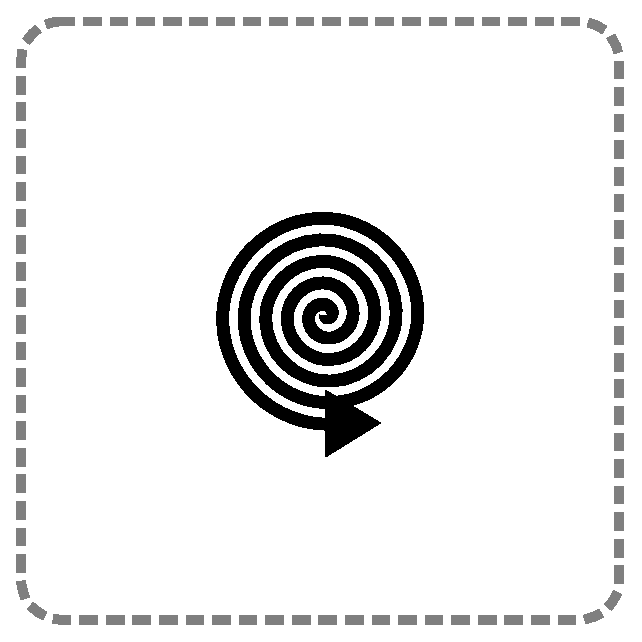
\includegraphics[width = 4cm]{figures/teachLogo/sspiral.eps}
    \end{columns}
  }
  \visible<9>{
    \vspace{0.2cm}
    \texttt{\alert{NUM} ::= 1 | $\pi$ | $\infty$ | $\varepsilon$ | + | - | * | / }
  }
\end{frame}

\begin{frame}{Turtle graphics --- Training tasks}
  \centering
  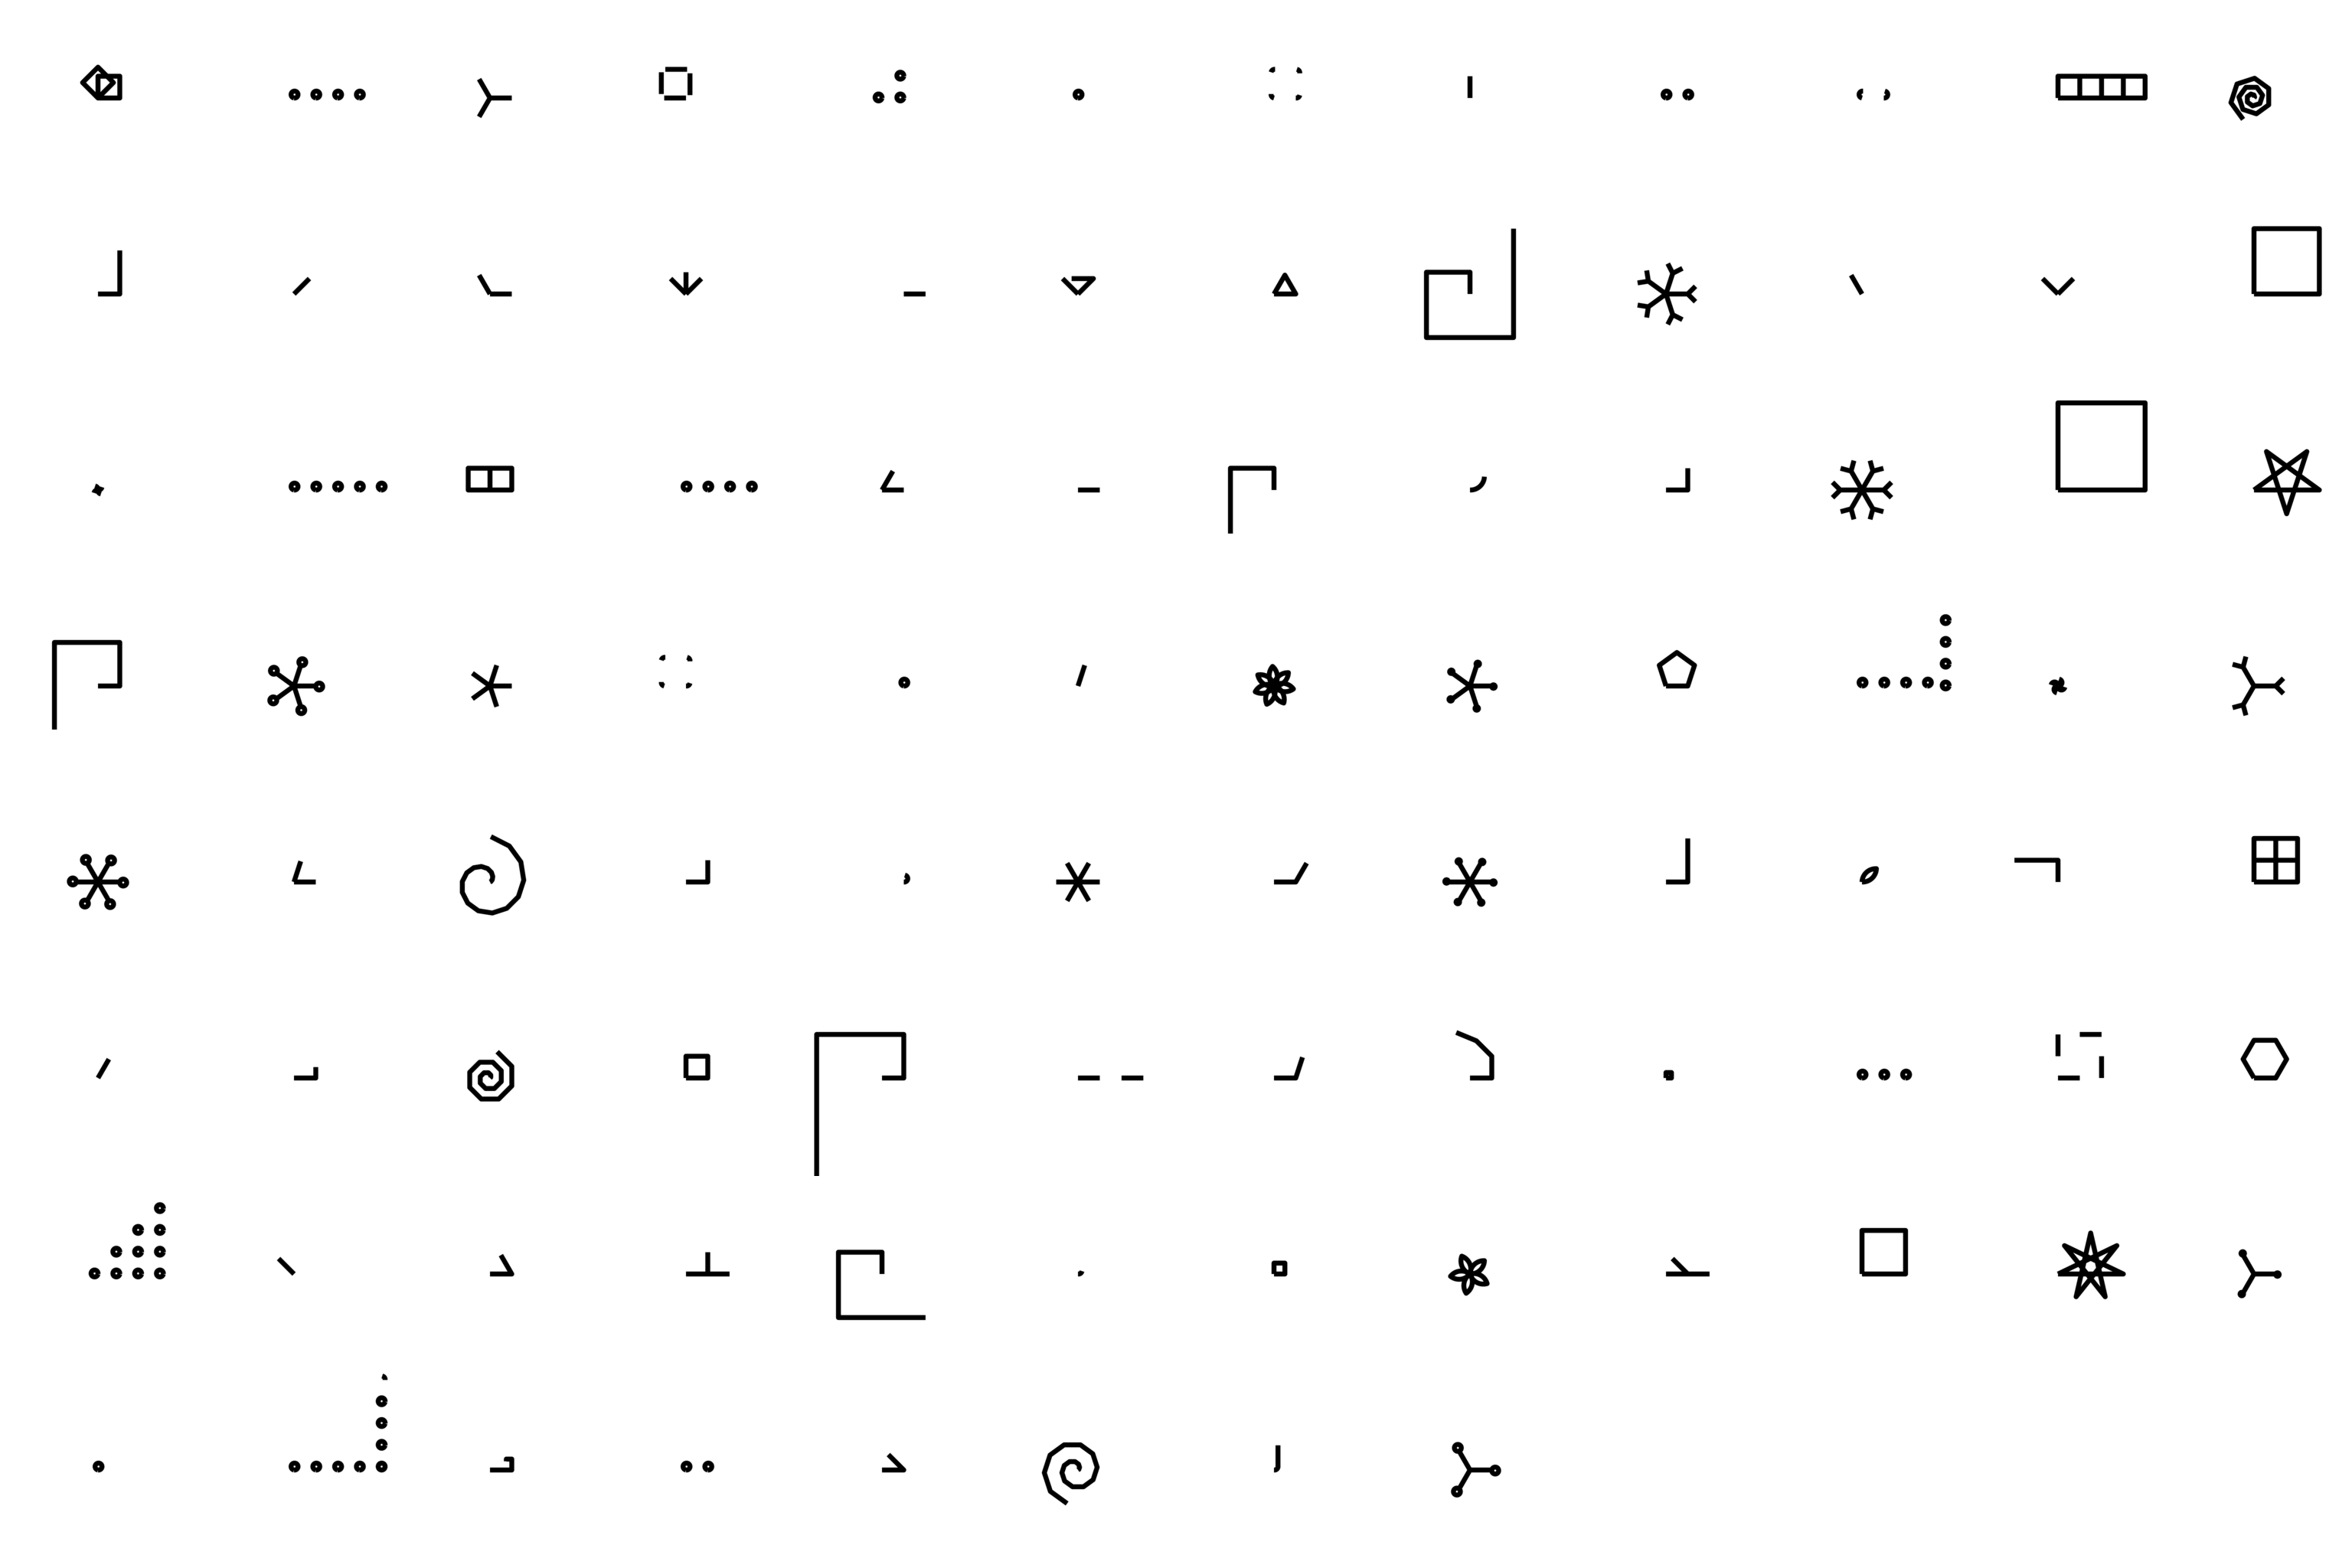
\includegraphics[width=11cm]{figures/tasksMinusBehaviour.png}
\end{frame}

\begin{frame}{Contributions}

  \textbf{Takeaway:}
  \begin{itemize}
    \item Humans flexibly adapt to diverse sets of new problem domains --- DreamCoder takes a step in this direction
  \end{itemize}
  \pause

  \textbf{Future work}

  \begin{itemize}
  \item More human-like learning: intelligently composing new tasks, 
    \pause
  \item Theory learning
    \item Planning
    \end{itemize}

  \end{frame}

\end{document}
